\documentclass[11pt, a4paper, reqno]{scrartcl}

\usepackage[utf8]{inputenc}
\usepackage{a4wide}
\usepackage{libertine}
\usepackage{graphicx}
\usepackage{xcolor}
\usepackage{float}
\usepackage{amsmath}
\usepackage{microtype}
\usepackage{minted}

% for latex output of pandas
\usepackage{booktabs}

\begin{document}
    \title{Computational Statistics and Data Analysis\\Sheet No. 10}
    \author{David Bubeck, Patrick Nisbl\`e}
    \maketitle
    \section*{Problem 1: Higher-Order Fitting}

    For the first estimation of the linear fit coefficients by finding the slope a and intercept b to minimize the given formular we found:
    \begin{align*}
      a = 7.0\\
      b = 820
    \end{align*}

    Here is the printed summary of the lm function:

    \begin{minted}[
        fontsize=\footnotesize
      ]{r}
      lm(formula = metabolic.rate ~ body.weight, data = data)
    \end{minted}

    Output
    \begin{minted}[
        fontsize=\footnotesize
      ]{bash}
      Residuals:
          Min      1Q  Median      3Q     Max
      -245.74 -113.99  -32.05  104.96  484.81

      Coefficients:
                  Estimate Std. Error t value Pr(>|t|)
      (Intercept) 811.2267    76.9755  10.539 2.29e-13 ***
      body.weight   7.0595     0.9776   7.221 7.03e-09 ***
      ---
      Signif. codes:  0 ‘***’ 0.001 ‘**’ 0.01 ‘*’ 0.05 ‘.’ 0.1 ‘ ’ 1

      Residual standard error: 157.9 on 42 degrees of freedom
      Multiple R-squared:  0.5539,	Adjusted R-squared:  0.5433
      F-statistic: 52.15 on 1 and 42 DF,  p-value: 7.025e-09
    \end{minted}

    To compare these to methods we can see in the plot that it's actually quite good.

    Also the prediction for body weights of 150 and 200 kg we found with predict:
    \begin{minted}{bash}
      150 kg: 1870.156 with error estimation of 77.1995
      200 kg: 2223.132 with error estimation of 124.6124
    \end{minted}

    Code:
    \inputminted[
        fontsize=\footnotesize,
        linenos
      ]{r}{exercise_10_1.r}

    Plots:
    \begin{figure}[H]
      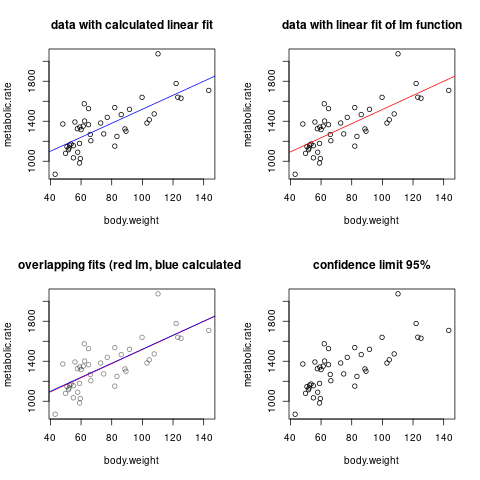
\includegraphics[width=.8\textwidth]{exercise_10_1.png}
      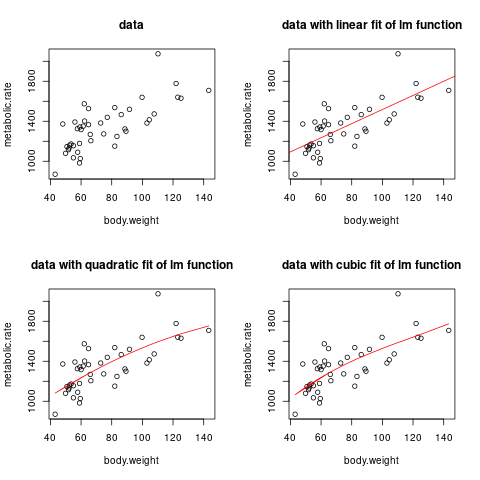
\includegraphics[width=.8\textwidth]{exercise_10_lm}
    \end{figure}

    \section*{Problem 2: linear fitting with errors}

    Code:
    \inputminted[
        fontsize=\footnotesize,
        linenos
      ]{r}{Exercise10_2.r}

    \begin{figure}[H]
      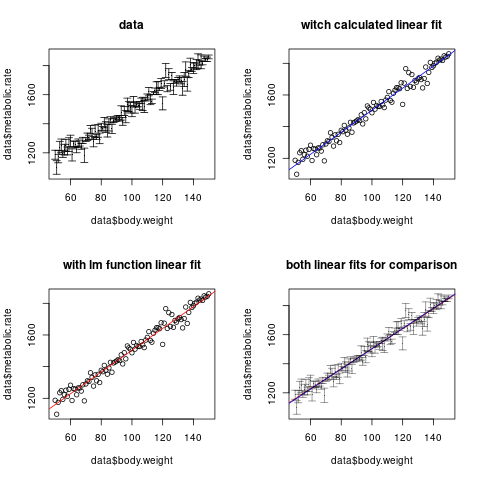
\includegraphics[width=\textwidth]{exercise10_2}
    \end{figure}
\end{document}
